\documentclass{beamer}

\newcommand{\isdef}{\hbox{$\stackrel{\mbox{\tiny def}}{=}$}}
\newcommand{\Dt}{\mathcal{D}}
\newcommand{\Reg}{\mathcal{R}}
\newcommand{\Pst}{\mathcal{P}}
\newcommand{\Trn}{\mathcal{T}}
\newcommand{\Kln}{\mathcal{K}}
\newcommand{\TrnA}{\Trn_{a}}
\newcommand{\EKnows}{\mathbf{EKnows}}
\newcommand{\Knows}{\mathbf{Knows}}
\newcommand{\CKnows}{\mathbf{CKnows}}
\newcommand{\KnowsZ}{\mathbf{Knows_{0}}}
\newcommand{\PKnowsZ}{\mathbf{PKnows_{0}}}
\newcommand{\PKnows}{\mathbf{PKnows}}
\newcommand{\KTrans}{\mathbf{KDo}}
\newcommand{\KDo}{\mathbf{KDo}}
\newcommand{\EDo}{\mathbf{EDo}}
\newcommand{\vars}[1]{\bar{#1}}
\newcommand{\PbU}{PbU}

\mode<presentation>{\usetheme{Dresden}}

\usepackage{fancyvrb}
\usepackage{bibentry}
\usepackage{tikz}

\title{Asynchronous Multi-Agent Domains\\ in the Situation Calculus}
\author[Ryan Kelly]{Ryan Kelly\\ Supervisor: Adrian Pearce}

\begin{document}

\begin{frame}
  \titlepage
\end{frame}

\begin{frame}
  \frametitle{Contributions}
  Powerful extensions to the Situation Calculus for representing and reasoning
  about rich, asynchronous multi-agent domains:
  \ \\
  \ \\
  \begin{itemize}
  \item Multi-agent Golog with distributed execution planning
  \item Reasoning about knowledge with hidden actions
  \item Techniques for effective inductive reasoning
  \item Reasoning about group-level knowledge modalities
  \item Planning joint executions with partial observability
  \end{itemize}
\end{frame}

\section{Situation Calculus}

\begin{frame}
\frametitle{The Situation Calculus}
A formalism for reasoning about dynamic worlds.
\ \\
\ \\
\emph{Actions} are instantaneous events causing the world to change
\begin{itemize}
  \item $pickup(Thomas,Bowl)$
\end{itemize}
\ \\
\ \\
\emph{Situations} are histories of actions that have been performed
\begin{itemize}
  \item $S_0$,\ \ $do(pickup(Harriet,Knife),S_0)$
\end{itemize}
\ \\
\ \\
\emph{Fluents} are situation-dependent properties of the world
\begin{itemize}
  \item $Poss(a,s)$,\ \ $Holding(Harriet,Knife,s)$
\end{itemize}
\end{frame}

\begin{frame}
\frametitle{The Situation Calculus}
\emph{Successor State Axioms} define what holds after an action in terms of what held before the action
\begin{itemize}
  \item $Holding(agt,obj,do(a,s)) \equiv a = pickup(agt,obj)$ \\
        $\,\,\,\,\,\,\,\,\,\,\,\,\,\vee Holding(agt,obj,s) \wedge \neg\left(a = drop(agt,obj)\right)$
\end{itemize}
\ \\
\ \\
\pause
From these components we can built a first-order \emph{Theory of Action}
with which agents can:
\begin{itemize}
  \item Reason about when actions are possible
  \item Reason about the effects of actions
  \item Represent sequences of actions as situations:\[
\left[a_1, a_2, a_3, a_4\right] \rightarrow do(a_4,do(a_3,do(a_2,do(a_1,S_0))))
\]
\end{itemize}
\end{frame}

\begin{frame}
\frametitle{Golog}
Golog introduces programming to the situation calculus.\\
Primitive actions are composed using operators such as:

\begin{itemize}
  \item $a$ - Perform a primitive action
  \item $\delta_1;\delta_2$ - Perform two programs in sequence
  \item $\phi?$ - Assert that a condition holds
  \item $\delta_1|\delta_2$ - Choose between programs to execute
  \item $\pi(x,\ \delta(x))$ - Choose suitable bindings for variables
  \item $\delta^*$ - Execute a program zero or more times
  \item $\delta_1 || \delta_2$ - Execute programs concurrently
\end{itemize}
\ \\
\ \\
\pause
Key Point:  programs can include \alert{nondeterminism}
\end{frame}

\begin{frame}
\frametitle{A Quick Example}
Consider a Golog program for getting to uni of a morning:\[
\begin{array}{c}
ringAlarm;(hitSnooze; ringAlarm)^*;turnOffAlarm;\\
\pi(food,\ edible(food)?;eat(food)); (haveShower || brushTeeth);\\
(driveToUni\ |\ trainToUni); (time<9:00)?
\end{array}\]

There are potentially many ways to execute this program, depending on which 
actions are possible in the world.
\pause
\ \\
\ \\
Use theory of action to plan a \emph{Legal Execution}:\[
\Dt \models \exists s,\delta': Trans^{*}(\delta,S_0,\delta',s) \wedge Final(\delta',s)\]

\end{frame}

\begin{frame}
\frametitle{Why the Situation Calculus?}
\begin{itemize}
\item Elegant, monotonic solution to frame problem
\item Effective reasoning techniques based on Regression
\item Straightforward implementation as a logic program
\item Powerful nondeterminism control for programming/planning
\item Large body of existing work and results
\item Many useful extensions for rich domain features...
\end{itemize}
\end{frame}

\begin{frame}
\frametitle{Extending the Situation Calculus}
\begin{itemize}
\pause
\item Concurrent Actions:\ \ \ $do(\{a_1,a_2\},s)$
\pause
\item Continuous time:\ \ \ $do(c,t,s)$
\pause
\item Long-running tasks:\ \ \ $begin(t)$, $doing(t,s)$, $end(t)$
\pause
\item Natural processes:\ \ \ $Legal(a,s)\rightarrow\neg\exists n: nat(n) \wedge Poss(n,s)$
\pause
\item Incomplete knowledge:\ \ \ $\Knows(\phi,s)$
\pause
\item Asynchronous multi-agent domains:\ \ \ ???
\end{itemize}
\ \\
\ \\
\pause
Our work continues this proud tradition.
\end{frame}

\section{MIndiGolog}

\begin{frame}
\frametitle{Motivating Example: The Cooking Agents}
Several robotic chefs inhabit a kitchen, along with various ingredients,
appliances and utensils.  They must cooperate to produce a meal consisting
of several dishes.\\
\ \\
\pause
\begin{columns}
  \begin{column}{0.5\textwidth}
\[
\pause
\begin{array}{c}
\mathbf{proc}\ MakeSalad(bowl)\\
(ChopTypeInto(Lettuce,bowl)\ ||\\
ChopTypeInto(Carrot,bowl)\ ||\\
ChopTypeInto(Tomato,bowl)\ )\ ;\\
\pi(agt, Mix(agt,bowl,1))\\
\mathbf{end}\end{array}\]
  \end{column}
  \begin{column}{0.5\textwidth}
\[
\pause
\begin{array}{c}
\mathbf{proc}\ ChopTypeInto(type,dest)\\
\pi((agt,obj), \ \ \ \ \ \ \ \\
IsType(obj,type)?\ ;\\
Chop(agt,obj)\ ;\\
PlaceIn(agt,obj,dest))\\
\mathbf{end}\end{array}\]
  \end{column}
\end{columns}
\end{frame}

\begin{frame}
\frametitle{MIndiGolog}
Vision:
\begin{itemize}
\item Agents cooperate to plan and perform the execution of a shared Golog program
\end{itemize}
\ \\
\ \\
Contributions
\begin{itemize}
\item Merge concurrent actions with concurrent program execution
\item Integrate time and natural actions for coordination
\item Share planning workload using distributed logic programming
\end{itemize}
\end{frame}

\begin{frame}
\frametitle{MIndiGolog Semantics}
Agents should take advantage of true concurrency. Basic idea:
\begin{multline*}
Trans(\delta_{1}||\delta_{2},s,\delta',s')\equiv\exists\gamma\,.\, Trans(\delta_{1},s,\gamma,s')\wedge\delta'=(\gamma||\delta_{2})\\
\shoveright{\vee\exists\gamma\,.\, Trans(\delta_{2},s,\gamma,s')\wedge\delta'=(\delta_{1}||\gamma)}\\
\end{multline*}
\end{frame}

\begin{frame}
\frametitle{MIndiGolog Semantics}
Agents should take advantage of true concurrency. Basic idea:
\begin{multline*}
Trans(\delta_{1}||\delta_{2},s,\delta',s')\equiv\exists\gamma\,.\, Trans(\delta_{1},s,\gamma,s')\wedge\delta'=(\gamma||\delta_{2})\\
\shoveright{\vee\exists\gamma\,.\, Trans(\delta_{2},s,\gamma,s')\wedge\delta'=(\delta_{1}||\gamma)}\\
\shoveright{\vee\exists c_{1},c_{2},\gamma_{1},\gamma_{2},t\,.\, Trans(\delta_{1},s,\gamma_{1},do(c_{1},t,s))\wedge}\\ 
Trans(\delta_{2},s,\gamma_{2},do(c_{2},t,s))\wedge\delta'=(\gamma_{1}||\gamma_{2})\wedge s'=do(c_{1}\cup c_{2},t,s)
\end{multline*}
\end{frame}

\begin{frame}
\frametitle{MIndiGolog Semantics}
Agents should take advantage of true concurrency. Basic idea:
\begin{multline*}
Trans(\delta_{1}||\delta_{2},s,\delta',s')\equiv\exists\gamma\,.\, Trans(\delta_{1},s,\gamma,s')\wedge\delta'=(\gamma||\delta_{2})\\
\shoveright{\vee\exists\gamma\,.\, Trans(\delta_{2},s,\gamma,s')\wedge\delta'=(\delta_{1}||\gamma)}\\
\shoveright{\vee\exists c_{1},c_{2},\gamma_{1},\gamma_{2},t\,.\, Trans(\delta_{1},s,\gamma_{1},do(c_{1},t,s))}\\
\shoveright{\wedge Trans(\delta_{2},s,\gamma_{2},do(c_{2},t,s))\wedge\delta'=(\gamma_1||\gamma_2)\wedge s'=do(c_1\cup c_2,t,s)}\\
\wedge Poss(c_1\cup c_2,t,s)\wedge\forall a.\left[a\in c_{1}\wedge a\in c_{2}\rightarrow Natural(a)\right]
\end{multline*}
\end{frame}

\begin{frame}
\frametitle{MIndiGolog Execution}
The semantics of Golog can be neatly encoded as a logic program.

Prolog is traditionally used.

We use Oz for its strong distributed programming support.

\VerbatimInput[fontsize=\scriptsize,frame=lines]{goloz_trans.oz}

\end{frame}

\begin{frame}
\frametitle{MIndiGolog Execution}
Using the builtin ParallelSearch object, the agents can transparently
share the planning workload:

\VerbatimInput[fontsize=\scriptsize,frame=lines]{goloz_do_parallel.oz}

\end{frame}

\begin{frame}
\frametitle{Example Output}
\begin{columns}
  \begin{column}{0.5\textwidth}
    \VerbatimInput[fontsize=\tiny]{output_makeSalad_1.txt}
  \end{column}
  \begin{column}{0.5\textwidth}
    \VerbatimInput[fontsize=\tiny]{output_makeSalad_2.txt}
  \end{column}
\end{columns}
\ \\
\ \\
\pause
Can give idle agents other work using:\[
MakeSalad(Bowl1)\ ||\ MakeCake(Bowl2)\ ||\ \dots\]
\end{frame}

\begin{frame}
\frametitle{Contribution}
\textbf{MIndiGolog:} a Golog semantics and implementation for shared program 
 execution by a team  of cooperating agents:
\begin{itemize}
\item Safely taking advantage of true concurrency
\item Automatically accounting for predictable environment behavior
\item Using distributed logic programming to share the workload
\end{itemize}
\end{frame}

\section{Asynchronicity}

\begin{frame}
\frametitle{Limitation: Synchronicity}
This works well, but it depends on two assumptions:
\begin{itemize}
\item Complete knowledge (linear plan, no sensing)
\item Synchronous domain (agents proceed in lock-step)
\end{itemize}
\pause
\ \\
\ \\
Nearly universal in the literature: "assume all actions are public".
\ \\
\ \\
\alert{Challenge:}  Regression depends intimately on synchronicity

\end{frame}

\begin{frame}
\frametitle{Regression}
Regression operates by unwinding actions one at a time:
\ \\
\ \\
$\Reg(Holding(agt,obj,do(c,s))) \Rightarrow$\\
$\,\,\,\,\,\,\,\,\,\,\,\,\,\,\,\,\,\,\,\,\,\,\,pickup(agt,obj) \in c$ \\
$\,\,\,\,\,\,\,\,\,\,\,\,\,\vee Holding(agt,obj,s) \wedge \neg\left(drop(agt,obj) \in c\right)$
\ \\
\ \\
\pause
By repeatedly applying it, we get a query about $S_0$:
\[
\Dt\models\phi[do(c_1,do(c_2,\dots,S_0))]\,\,\,\,\mathrm{iff}\,\,\,\,\Dt\models\Reg^{*}(\phi)[S_0]
\]
\ \\
\ \\
\pause
If you don't know the current situation, you cannot reason using regression.
\end{frame}

\begin{frame}
\frametitle{Observations}
First, we must represent asynchronicity.\\
We reify the \emph{observations} made by each agent:
\ \\
\ \\
\small
$Obs(agt,c,s) = o$
\ \\
\ \\
\pause
$View(agt,S_0) = \epsilon$\\
$Obs(agt,c,s) = \{\} \rightarrow View(agt,do(c,s)) = View(agt,s)$\\
$Obs(agt,c,s) \neq \{\} \rightarrow View(agt,do(c,s)) = Obs(agt,c,s) \cdot View(agt,s)$
\normalsize
\ \\
\ \\
\pause
If $Obs(agt,c,s)=\{\}$ then the actions are completely hidden.
\end{frame}

\begin{frame}
\frametitle{Observations}
In synchronous domains, everyone observes every action:
\begin{equation*}
a \in Obs(agt,c,s)\ \equiv\ a \in c
\end{equation*}
\pause
Sensing results can be easily included:
\begin{equation*}
a\#r \in Obs(agt,c,s)\ \equiv\ a \in c \wedge SR(a,s)=r
\end{equation*}
\pause
And observability can be axiomatised explicitly
\begin{equation*}
a \in Obs(agt,c,s)\ \equiv\ a \in c \wedge CanObs(agt,a,s)
\end{equation*}
\end{frame}

\begin{frame}
\frametitle{Observations}
Action:  global event changing the state of the world\\
Observation:  local event changing an agent's knowledge
\ \\
\ \\
Situation:  global history of actions giving current world state\\
View:  local history of observations giving current knowledge
\ \\
\ \\
\pause
How can we let agents reason using only their local view?
\end{frame}

\section{Knowledge}

\begin{frame}
\frametitle{Knowledge}
If an agent is unsure about the state of the world, there must be several
different states of the world that it considers possible.

The agent \emph{knows} $\phi$ iff $\phi$ is true in all possible worlds.
\begin{center}
  \includegraphics[scale=0.3]{poss_worlds}
\end{center}
\begin{equation*}
\mathbf{Knows}(Q)\ \wedge\ \neg\mathbf{Knows}(P)\ \wedge\ \neg\mathbf{Knows}(R)\ \wedge\ \mathbf{Knows}(P \vee R)
\end{equation*}

\end{frame}

\begin{frame}
\frametitle{Knowledge}
Introduce a possible-worlds fluent $K(agt,s',s)$:

\begin{center}
  \includegraphics[scale=0.4]{k_relation}
\end{center}

We can then define knowledge as a simple macro:
\[ \mathbf{Knows}(agt,\phi,s)\ \isdef\ \forall s'\left[K(agt,s',s)\rightarrow \phi(s')\right] \]
\end{frame}

\begin{frame}
\frametitle{Knowledge follows Observation}
Halpern \& Moses, 1990:\\
"an agent's knowledge at a given time must depend only on its local history:
the information that it started out with combined with the events it has
observed since then"
\pause
\ \\
\ \\
Clearly, we require:
\begin{equation*}
K(agt,s',s)\ \equiv\ View(agt,s') = View(agt,s)
\end{equation*}
We must enforce this in the successor state axiom for $K$.
\end{frame}

\begin{frame}
\frametitle{Knowledge: The Synchronous Case}
\begin{center}
  \includegraphics[scale=0.4]{frame_soln}
\end{center}
\end{frame}

\begin{frame}
\frametitle{Knowledge: The Synchronous Case}
In the synchronous case, $K_0$ has a simple successor state axiom:
\begin{multline*}
 K_0(agt,s'',do(c,s)) \equiv \exists s',c':\ s''=do(c',s') \wedge K_0(agt,s',s)\\
  \wedge Poss(c',s') \wedge Obs(agt,c,s) = Obs(agt,c',s')
\end{multline*}
\ \\
\ \\
\pause
And a correspondingly simple regression rule:
\begin{multline*}
 \Reg(\KnowsZ(agt,\phi,do(c,s))\ \isdef\ \exists o: Obs(agt,c,s)=o\\
  \wedge \forall c': \KnowsZ(agt,Poss(c')\wedge Obs(agt,c')=o \rightarrow \Reg(\phi,c'))
\end{multline*}
\end{frame}

\begin{frame}
\frametitle{Knowledge: The Asynchronous Case}
\begin{center}
  \includegraphics[scale=0.3]{k_unobs}
\end{center}
\end{frame}

\begin{frame}
\frametitle{Knowledge: The Asynchronous Case}
First, some notation:
\begin{equation*}
  s <_{\alpha} do(c,s')\ \equiv\ s \leq_{\alpha} s' \wedge \alpha(c,s')
\end{equation*}
\begin{equation*}
  PbU(agt,c,s)\ \isdef\ Poss(c,s) \wedge Obs(agt,c,s) = \{\}
\end{equation*}
\pause
\ \\
Then the intended dynamics of knowledge update are:
\begin{multline*}
  K(agt,s'',do(c,s))\ \equiv\ \exists o: Obs(agt,c,s) = o  \\
  \wedge \left[o = \{\} \rightarrow K(agt,s'',s)\right] \\
  \wedge \left[o \neq \{\} \rightarrow \exists c',s': K(agt,s',s)\right. \\
  \left.\wedge Obs(agt,c',s') = o \wedge Poss(c',s') \wedge do(c',s') \leq_{PbU(agt)} s''\right]
\end{multline*}
\end{frame}

\begin{frame}
\frametitle{Sync vs Async}
We've gone from this:
\begin{multline*}
 K_0(agt,s'',do(c,s)) \equiv \exists s',c':\ s''=do(c',s') \wedge K_0(agt,s',s)\\
  \wedge Poss(c',s') \wedge Obs(agt,c,s) = Obs(agt,c',s')
\end{multline*}
\pause
To this:
\begin{multline*}
  K(agt,s'',do(c,s))\ \equiv\ \exists o: Obs(agt,c,s) = o  \\
  \wedge \left[o = \{\} \rightarrow K(agt,s'',s)\right] \\
  \wedge \left[o \neq \{\} \rightarrow \exists c',s': K(agt,s',s)\right. \\
  \left.\wedge Obs(agt,c',s') = o \wedge Poss(c',s') \wedge do(c',s') \leq_{PbU(agt)} s''\right]
\end{multline*}
\pause
It's messier, but it's also hiding a much bigger problem...
\end{frame}

\begin{frame}
\frametitle{Regressing Knowledge}
Our new SSA uses $\leq_{PbU(agt)}$  to quantify over all future situations.  Regression cannot be applied to such an expression.
\ \\
\ \\
An asynchronous account of knowledge \alert{cannot} be approached using
the standard regression operator.
\ \\
\ \\
\pause
In fact, this quantification requires a second-order induction axiom.

Must we abandon hope of an effective reasoning procedure?
\end{frame}

\begin{frame}
\frametitle{Property Persistence}
Suppose we could "factor out" the quantification. Then we could get
on with the business of doing regression.
\ \\
\ \\
Define the \emph{persistence condition} $\mathcal{P}[\phi,\alpha]$ of a formula
 $\phi$ and action conditions $\alpha$ to mean: assuming all future actions
satisfy $\alpha$, $\phi$ will remain true.
\begin{equation*}
  \mathcal{P}[\phi,\alpha](s)\ \equiv\ \forall s': s \leq_{\alpha} s' \rightarrow \phi(s')
\end{equation*}
Like $\mathcal{R}$, the idea is to transform a query into a form that is easier
to deal with.
\end{frame}

\begin{frame}
\frametitle{Property Persistence}
The persistence condition can be calculated as a fixpoint:
\begin{equation*}
  \Pst^{1}[\phi,\alpha](s)\ \isdef\ \phi(s) \wedge \forall c: \alpha(c) \rightarrow \phi(do(c,s))
\end{equation*}
\begin{equation*}
  \Pst^{n}[\phi,\alpha](s)\ \isdef\ \Pst^{1}[\Pst^{n-1}[\phi,\alpha],\alpha]
\end{equation*}
\ \\
\ \\
\pause
\begin{equation*}
  \left(\Pst^{n}[\phi,\alpha] \rightarrow \Pst^{n+1}[\phi,\alpha]\right) \Rightarrow \left(\Pst^{n}[\phi,\alpha] \equiv \Pst[\phi,\alpha]\right)
\end{equation*}
\ \\
\ \\
This calculation can be done using \emph{static domain reasoning} and provably terminates in several important cases.
\end{frame}

\begin{frame}
\frametitle{Regressing Knowledge}
\begin{center}
  \includegraphics[scale=0.3]{k_unobs_highlighted}
\end{center}
\end{frame}

\begin{frame}
\frametitle{Regressing Knowledge}
It becomes possible to define the regression of our $\mathbf{Knows}$ macro:
\begin{multline*}
  \mathcal{R}[\mathbf{Knows}(agt,\phi,do(c,s))] = \\
     \left[ Obs(agt,c,s) = \{\} \rightarrow \mathbf{Knows}(agt,\phi,s) \right] \\
     \wedge \left[ \exists o : Obs(agt,c,s) = o \wedge o\neq \{\} \rightarrow \right. \\
     \mathbf{Knows}(agt,\forall c' : Obs(agt,c')=o \rightarrow \\
     \left.\mathcal{R}[\mathcal{P}[\phi,PbU(agt)](do(c',s'))],s)\right]
\end{multline*}
\end{frame}

\begin{frame}
\frametitle{View-Based Reasoning}
The regression operator can be modified to act over observation histories,
instead of over situations:
\begin{multline*}
  \mathcal{R}[\mathbf{Knows}(agt,\phi,o \cdot h)] = \\
  \mathbf{Knows}(agt,\forall c' : Obs(agt,c',s')=o \rightarrow \\
     \mathcal{R}[\mathcal{P}[\phi,PbU(agt)](do(c',s'))],h)
\end{multline*}
We can equip agents with a situation calculus model of their own environment.
\end{frame}


\begin{frame}
\frametitle{Contribution}
\textbf{Persistence Condition:}  a new technique for inductive reasoning
\begin{itemize}
\item Using restricted forms of domain reasoning
\item Built on, and interacting well with, standard regression
\item Allowing the inductive component to be "factored out" of other reasoning tasks
\end{itemize}
\end{frame}

\begin{frame}
\frametitle{Contribution}
A robust account of \textbf{knowledge} based on observations, allowing for
arbitrarily-long sequences of hidden actions.
\begin{itemize}
\item That subsumes existing accounts of knowledge
\item With regression rules utilising the persistence condition
\item Allowing agents to reason about their own knowledge using only their local information
\end{itemize}
\end{frame}

\section{Group Knowledge}

\begin{frame}
\frametitle{Group-Level Knowledge}
The basic group-level operator is "Everyone Knows":
\begin{gather*}
\mathbf{EKnows}(G,\phi,s)\ \isdef \bigwedge_{agt \in G} \mathbf{Knows}(agt,\phi,s)\\
\mathbf{EKnows}^{2}(G,\phi,s)\ \isdef\ \mathbf{EKnows}(G,\mathbf{EKnows}(G,\phi),s)\\
\dots \\
\mathbf{EKnows}^{n}(G,\phi,s)\ \isdef\ \mathbf{EKnows}(G,\mathbf{EKnows}^{n-1}(G,\phi),s)
\end{gather*}
\pause
Eventually, we get "Common Knowledge":
\begin{gather*}
\mathbf{CKnows}(G,\phi,s)\ \isdef\ \mathbf{EKnows}^{\infty}(agt,\phi,s)
\end{gather*}
\end{frame}

\begin{frame}
\frametitle{Regressing Group Knowledge}
Since $\mathbf{EKnows}$ is finite, it can be expanded to perform regression.
\ \\
\ \\
$\mathbf{CKnows}$ is infinitary, so this won't work for common knowledge.

We need to regress it directly.\pause Maybe like this?
\begin{multline*}
\mathcal{R}[\mathbf{CKnows}(G,\phi,do(c,s))]\ \isdef \\
\exists o: \mathbf{CObs}(G,c,s)=o\ \wedge\\
\forall c': \mathbf{CKnows}(G,Poss(c') \wedge \mathbf{CObs}(agt,c')=o \rightarrow \mathcal{R}[\phi[do(c',s)]],s)
\end{multline*}
\ \\
\ \\
\pause
It is \alert{impossible} to express $\mathcal{R}[\mathbf{CKnows}]$ in terms of $\mathbf{CKnows}$
\end{frame}

\begin{frame}
\frametitle{Regressing Group Knowledge}
\begin{center}
  \includegraphics[scale=0.35]{pk_regression}
\end{center}
\end{frame}

\begin{frame}
\frametitle{Epistemic Path Language}
$\Reg[\CKnows]$ requires a more expressive epistemic language.
\ \\
\ \\
Dynamic Logics are formalisms for building programs from actions:
\begin{gather*}
A\ ;\ ?Poss(B)\ ;\ B \\
A\ ;\ (B \cup C) \\
A^*\ ;\ ?Done \\
x:=?\ ;\ ?Avail(x)\ ;\ pickup(X)
\end{gather*}
But they don't \emph{have} to be interpreted over actions.\\
More generally, DLs are logics of \emph{paths}.
\end{frame}

\begin{frame}
\frametitle{Epistemic Path Language}
Idea from van Bentham, van Eijck and Kooi.\\
"Logics of Communication and Change", Info. \& Comp., 2006
\ \\
\ \\
We can interpret Dynamic Logic epistemically:
\begin{gather*}
\mathbf{KDo}(agt,s,s')\ \isdef\ K(agt,s',s)\\
\mathbf{KDo}(?\phi,s,s')\ \isdef\ s'=s \wedge \phi[s]\\
\mathbf{KDo}(\pi_1;\pi_2,s,s')\ \isdef\ \exists s'': \mathbf{KDo}(\pi_1,s,s'') \wedge \mathbf{KDo}(\pi_2,s'',s')\\
\mathbf{KDo}(\pi_1\cup\pi_2,s,s')\ \isdef\ \mathbf{KDo}(\pi_1,s,s'') \vee \mathbf{KDo}(\pi_2,s,s')\\
\mathbf{KDo}(\pi^*,s,s')\ \isdef\ \mathrm{refl. tran. closure}\left[\mathbf{KDo}(\pi,s,s'')\right]\\
\end{gather*}
\end{frame}

\begin{frame}
\frametitle{Epistemic Path Language}
New macro for path-based knowledge:
\begin{equation*}
\mathbf{PKnows}(\pi,\phi,s)\ \isdef\ \forall s': \mathbf{KDo}(\pi,s,s') \rightarrow \phi[s']
\end{equation*}
Used like so:
\begin{gather*}
\mathbf{Knows}(agt,\phi,s)\ \equiv\ \mathbf{PKnows}(agt,\phi,s)\\
\mathbf{Knows}(agt_1,\mathbf{Knows}(agt_2,\phi),s)\ \equiv\ \mathbf{PKnows}(agt_1 ; agt_2,\phi,s)\\
\mathbf{EKnows}(G,\phi,s)\ \equiv\ \mathbf{PKnows}(\bigcup_{agt \in G}agt,\phi,s)\\
\mathbf{CKnows}(G,\phi,s)\ \equiv\ \mathbf{PKnows}((\bigcup_{agt \in G}agt)^*,\phi,s)
\end{gather*}
\end{frame}

\begin{frame}
\frametitle{Regressing Epistemic Paths}
It's now possible to formulate a regression rule for $\mathbf{PKnows}$ in synchronous domains:
\begin{multline*}
\Reg[\mathbf{PKnows_0}(\pi,\phi,do(c,s))] \Rightarrow \\
 \forall c': \mathbf{PKnows_0}(\Trn[\pi,c,c'],\Reg[\phi(c')],s)
\end{multline*}
$\mathcal{T}$ basically encodes the semantics of $\mathbf{KDo}$
\begin{gather*}
\mathcal{T}\{agt\}\ \isdef\ \mathrm{s.s.a.\ for}\ K\ \mathrm{fluent} \\
\mathcal{T}\{?\phi\}\ \isdef\ ?\mathcal{R}\{\phi\} \\
\mathcal{T}\{\pi_1\cup\pi_2\}\ \isdef\ \mathcal{T}\{\pi_1\}\cup\mathcal{T}\{\pi_2\} \\
\mathcal{T}\{\pi^*\} \isdef\ \mathcal{T}\{\pi\}^*
\end{gather*}
\end{frame}

\begin{frame}
\frametitle{Asynchronicity}
We can "fake" asynchronicity using $\mathbf{PKnows_0}$ and a stack of empty actions:
\begin{gather*}
\mathcal{E}[do(c,s)]\ \isdef\ do(\{\},do(c,\mathcal{E}[s])) \\
\mathcal{E}^n[s] \isdef\ \mathcal{E}[\mathcal{E}^{n-1}[s]]
\end{gather*}
Using a fixpoint construction that mirrors $\Pst$, define:
\begin{equation*}
\mathbf{PKnows}(\pi,\phi,s)\ \isdef\ \mathbf{PKnows_0}(\pi,\phi,\mathcal{E}^{\infty}[s])
\end{equation*}
We prove that $\mathbf{PKnows}(agt,\phi,s) \equiv \mathbf{Knows}(agt,\phi,s)$
\end{frame}

\begin{frame}
\frametitle{Contribution}
\textbf{Complex Epistemic Modalities:}  an encoding of group-level knowledge using the syntax of dynamic logic
\begin{itemize}
\item Built entirely use macro-expansion
\item In which common knowledge is amenable to regression
\item Incorporating arbitrarily-long sequences of hidden actions
\end{itemize}
\end{frame}

\section{Joint Execution}

\begin{frame}
\frametitle{Joint Executions}
The Golog execution planning process produces a \emph{situation} representing
a legal execution of the program.
\ \\
\ \\
This is a \emph{linear} and \emph{fully-ordered} sequence of actions, 
demanding total synchronicity during execution.
\ \\
\ \\
Multiple agents should be able to execute independent actions independently.
\begin{itemize}
\item need a \emph{partially-ordered} representation
\end{itemize}
\end{frame}

\begin{frame}
\frametitle{Prime Event Structures}
Prime event structures are a canonical representation for partially-ordered
branching sequences of events:
\begin{itemize}
\item A set of events, $\mathcal{V}$
\item A partial order on events, $e_1 \prec e_2$
\item A conflict relation, $e_1 \# e_2$
\item A labelling function, $\gamma(e) = lbl$
\end{itemize}
\ \\
\ \\
Define \emph{enablers} and \emph{alternatives} as follows:
\begin{itemize}
\item $j\in ens(i)\equiv j\prec i\,\wedge\,\forall k\in ens(i):\,\neg(j\prec k)$
\item $j\in alts(i)\equiv j \# i\,\wedge\,\forall k\in ens(i):\,\neg(j \# k)$
\end{itemize}
\end{frame}

\begin{frame}
\frametitle{Joint Executions}
\begin{center}
  \includegraphics[scale=0.31]{jointexec}
\end{center}
\end{frame}

\begin{frame}
\frametitle{Joint Executions}
We enforce several restrictions to ensure a JE can always be executed.
\ \\
\ \\
\begin{itemize}
\item Independent events have independent actions
\item Every canonical history is legal
\item All possible outcomes are considered
\item Actions are enabled by observable events:
\item Overlapping views enable identical actions:
\end{itemize}
\end{frame}

\begin{frame}
\frametitle{Planning with Joint Executions}
Our implementation maintains these restrictions while building a JE one action 
at a time - just like an ordinary situation term.

\VerbatimInput[fontsize=\scriptsize,frame=lines]{jeplan.oz}

\end{frame}

\begin{frame}
\frametitle{Planning with Joint Executions}

\begin{center}
  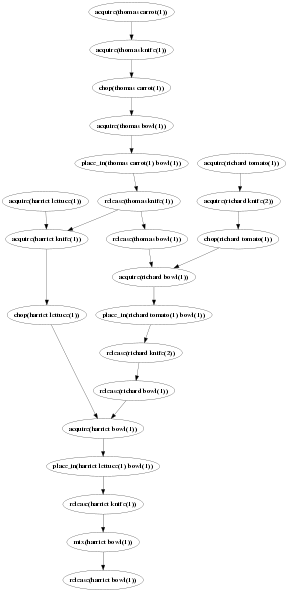
\includegraphics[scale=0.31]{plan}
\end{center}

\end{frame}

\begin{frame}
\frametitle{Contribution}
\textbf{Joint Execution:}  a partially-ordered data structure representing actions to be performed by a group of agents
\begin{itemize}
\item That ensures synchronisation is always possible
\item That can be reasoned about using standard sitcalc techniques
\item That can replace situation terms in the Golog planning process
\item Implemented in a MIndiGolog execution planner
\end{itemize}
\end{frame}

\section{Conclusions}

\begin{frame}
  \frametitle{Summary}
  \begin{itemize}
  \item Semantics for a multi-agent Golog variant, and an implementation allowing distributed execution planning.
  \item An account of hidden and partially-observable actions, in which agents can reason about their own knowledge using only their local information.
  \item A new meta-operator allowing regression rules that quantify over all future situations.
  \item A formal account of common knowledge that is amenable to effective automated reasoning using regression rules.
  \item A data structure for building partially-ordered branching sequences of actions during Golog execution planning.
  \end{itemize}
\end{frame}

\begin{frame}
\frametitle{Publications}
\small
\nocite{kelly06hlp_dps}
\nocite{kelly07sc_persistence}
\nocite{kelly07sc_know_obs}
\nocite{kelly08complex_epistemic_modalities}
\bibliographystyle{unsrt}
\bibliography{../../library/references}
\normalsize
\end{frame}

\begin{frame}
\centering \large Thank You\\
\end{frame}


\end{document}
